%%%%%%%%%%%%%%%%%%%%%%%%%%%%%%%%%%%%%%%%%%%%%%%%%%%%%%%%%%%
% | - Active Learning Machine Learning Methodology %%%%%%%%
% %%%%%%%%%%%%%%%%%%%%%%%%%%%%%%%%%%%%%%%%%%%%%%%%%%%%%%%%%
% Outline:
%   * PARAGRAPH 00
%     - General introduction and high-level overview of algorithm
%   * PARAGRAPH 01
%     - Candidate space generation methodology
%   * PARAGRAPH 02
%     - Quick paragraph about structure featurization
%   * PARAGRAPH 03
%     - Iterative AL algorithm procedure
%   * PARAGRAPH 04
%
%
%
%   * There will not be much motivation for our general approach from the introduction, so this is a good place to more properly layout our arguments
%
% Points to mention:
%   * Active learning frameworks are a means by which to generate the most valuable training data set, on the fly.
%   * The search space of materials is not a continuous space but a discrete array of individual structures
%
% TODO:
% __| %%%%%%%%%%%%%%%%%%%%%%%%%%%%%%%%%%%%%%%%%%%%%%%%%%%%%



% %%%%%%%%%%%%%%%%%%%%%%%%%%%%%%%%%%%%%%%%%%%%%%%%%%%%%%%%%
% ####################### Paragraph #######################
% %%%%%%%%%%%%%%%%%%%%%%%%%%%%%%%%%%%%%%%%%%%%%%%%%%%%%%%%%
% General intro to AL scheme
%
% %%%%%%%%%%%%%%%%%%%%%%%%%%%%%%%%%%%%%%%%%%%%%%%%%%%%%%%%%
% | - %%%%%%%%%%%%%%%%%%%%%%%%%%%%%%%%%%%%%%%%%%%%%%%%%%%%%
%
%Here, we present an active learning accelerated methodology for discovering novel and stable crystal polymorphs.
%
Our approach utilizes an active learning framework and makes use of a surrogate-model,
whereby a regression model is trained on a set of candidate materials by iteratively and intelligently sampling structures from a candidate set.
%
Figure~\ref{fig:all_diagram} gives an overview of the algorithm.% is presented in Figure~\ref{fig:all_diagram}.
%
There are two primary components of the algorithm, the first is the generation of the candidate space,
which defines the list of candidate crystal structures to be searched through (see Figure~\ref{fig:all_diagram}.a).
%
The structures within the candidate space are then transformed into a numerical vector representation for use in  a machine learning regression model.
%
The second component is the iterative search through candidate space via a continuously retrained surrogate model, (Figure~\ref{fig:all_diagram}.b).
% __| %%%%%%%%%%%%%%%%%%%%%%%%%%%%%%%%%%%%%%%%%%%%%%%%%%%%%

% %%%%%%%%%%%%%%%%%%%%%%%%%%%%%%%%%%%%%%%%%%%%%%%%%%%%%%%%%
% ####################### Paragraph #######################
% %%%%%%%%%%%%%%%%%%%%%%%%%%%%%%%%%%%%%%%%%%%%%%%%%%%%%%%%%
% CANDIDATE SPACE GENERATION
%
% %%%%%%%%%%%%%%%%%%%%%%%%%%%%%%%%%%%%%%%%%%%%%%%%%%%%%%%%%
% | - %%%%%%%%%%%%%%%%%%%%%%%%%%%%%%%%%%%%%%%%%%%%%%%%%%%%%
%The generation of the candidate space is a critical step in the discovery of novel crystal structures for a given system,
%since the initial candidate pool determines which structures that can ultimately be discovered, it is imperative to construct candidates that are sufficiently diverse, such that they encompass as much of the structural diversity in the PES as possible.
%
% TODO PENDING Ask @Ankit for these numbers
% The MP project number should be correct, but the OQMD number might be wrong
% MP{AB2: 2424, AB3: 2341} | OQMD{AB2: 4736, AB3: 28883}
Structures that comprise the candidate data sets for \IrOtwo and \IrOthree were constructed by first obtaining all \ABtwo and \ABthree structures in the Materials Project\cite{Jain2013} and OQMD\cite{Kirklin2015} databases
(in total \num{4528} \ABtwo and \num{23764} \ABthree entries).
%
To reduce the size of the candidate space while maintaining maximum structural diversity, structurally redundant systems were removed via a space-group based structural classification scheme developed by Jain \latin{et al.} \cite{Jain2018}.
Structural properties were defined by a unique combination of the element-nonspecific stoichiometry (\ABtwo, \ABthree, etc.), space group symmetry and Wyckoff positions, and are referred to as a materials structural prototype.
%
% This is my attempt to further clarify the previous sentence
Structures that share these properties are considered identical.
%
For example, the \num{300000} entry dataset of \ABOthree style perovskites in OQMD, which only differ by the choice of elements for A, B, and C, all belong to the same structural prototype.
%
Eliminating structurally redundant systems from the materials databases reduces the number of entries to \num{697} and \num{259} structures for the \ABtwo and \ABthree stoichiometries, respectively.
%
The orders of magnitude reduction between all structures and unique structures highlights the lack of structural diversity in the OQMD and MP databases.
%
To reduce the computational expense of the DFT calculations only bulk structures containing $\leq$ \num{75} atoms were included in the final candidate pool, further reducing the candidates spaces to \num{567} and \num{256} \ABtwo and \ABthree structures respectively.
%

We next substituted iridium and oxygen for the A and B sites, respectively,
and then used isotropic expansion/contraction of the unit cell to accommodate their atomic radii (further details in SI).  We then discarded an additional 87 structures with unreasonable Ir-O distances after cell volume optimization due to highly voluminous cells.
%
% NUMBER
%Because of the reasonable size of the reduced candidate space, and to validate our methods fully, we performed bulk relaxations for all \num{736} structures.
%
%
%Of the \num{823} structures, \num{736} were able to be fully optimized, while \num{87}, primarily \ABtwo structures were not able to be converged due to a variety of SCF convergence issues apparently due to highly voluminous cells.
%
The resulting candidate space was composed of \num{487} \IrOtwo and \num{249} \IrOthree structures, all of which have unique space group/Wyckoff combinations, ensuring their structural uniqueness.
We performed bulk relaxations of the cell vectors and atomic positions with DFT for all \num{736} structures for validation of our AL methodology. Further computational details of the DFT calculations can be found in the SI.
%
%While not particularly large in size, this data set will serve as a proof of concept.
%
%The candidate space size is ideal in that that we can tractably optimize each equilibrium structure for the entire dataset with DFT, thus allowing us to validate our AL approach.
%Further details on the isotropic cell expansion and DFT computational details can be found in the SI.
% __| %%%%%%%%%%%%%%%%%%%%%%%%%%%%%%%%%%%%%%%%%%%%%%%%%%%%%

% %%%%%%%%%%%%%%%%%%%%%%%%%%%%%%%%%%%%%%%%%%%%%%%%%%%%%%%%%
% ####################### Paragraph #######################
% %%%%%%%%%%%%%%%%%%%%%%%%%%%%%%%%%%%%%%%%%%%%%%%%%%%%%%%%%
% Short paragraph on featurization method
%
% %%%%%%%%%%%%%%%%%%%%%%%%%%%%%%%%%%%%%%%%%%%%%%%%%%%%%%%%%
% | - %%%%%%%%%%%%%%%%%%%%%%%%%%%%%%%%%%%%%%%%%%%%%%%%%%%%%
%
The candidate data set was featurized using the Voronoi tessellation fingerprinting scheme developed by Ward \latin{et al.} \cite{Ward2017} which produces a \num{271} length feature vector for each material that is invariant to isotropic expansions/contractions of the lattice, and somewhat insensitive to the exact atomic coordinates of the atoms.\cite{Ward2017}
%
These feature vectors encode both chemical and structural information by constructing attributes from elemental properties which are weighted by the local environment of the structure via the computation of the Voronoi decomposition of the cell lattice (Wigner-Seitz cell).
%
% How many columns of the 271 are redundant if stoich and composition are frozen
We applied the active learning model to the \IrOtwo and \IrOthree spaces separately, since we are interested in the most stable polymorphs for each stoichiometry.
%
Constraining the stoichiometry per application of the AL algorithm further reduces the \num{271} length  feature vector to \num{101} non-zero variance features.%,
%significantly reducing the dimensionality of the features.
%
% TODO Create cross-validation plot
Further dimensionality reduction was achieved via a principle component analysis (PCA) \cite{Tipping1999}, which was used to reduce the remaining \num{101} features to \num{10}, which, while only capturing ~80 percent of the variance in the features, demonstrated the optimal cross-validation error (see the Supporting Information).  \textbf{I'm a little dubious of this, where is it shown in SI?}
% __| %%%%%%%%%%%%%%%%%%%%%%%%%%%%%%%%%%%%%%%%%%%%%%%%%%%%%

% %%%%%%%%%%%%%%%%%%%%%%%%%%%%%%%%%%%%%%%%%%%%%%%%%%%%%%%%%
% ####################### Paragraph #######################
% %%%%%%%%%%%%%%%%%%%%%%%%%%%%%%%%%%%%%%%%%%%%%%%%%%%%%%%%%
% Active Learning Loop
%
% NOTE This paragraph is a bit long, find way to split into 2
% %%%%%%%%%%%%%%%%%%%%%%%%%%%%%%%%%%%%%%%%%%%%%%%%%%%%%%%%%
% | - %%%%%%%%%%%%%%%%%%%%%%%%%%%%%%%%%%%%%%%%%%%%%%%%%%%%%
%
The active learning algorithm proceeds through iterative generations of ML training, prediction, and acquisition steps that are visualized in Figure~\ref{fig:iro2_al}.
%
% COMBAK Did I get all of the important features of GP here? @Jose
To start, we utilized Gaussian process (GP) regression with Gaussian (or RBF) kernels as implemented in the CatLearn\cite{hansen2019atomistic,CatLearn_Repo} package for atomistic machine learning applications, and used it to train a regression model on a small seed set of DFT formation energies from randomly selected structures in the candidate space.
%
% NOTE I've introduced the aquis. crit. with the GP uncertainty before talking about aquis. in more detail, need to restructure
Herein, we utilized Gaussian process regression because they are highly flexible regression models which have built-in error quantification for each prediction.
%
The model is then used to predict the formation energies of the entire candidate space.
%
This predicted energy landscape is then used to select the next systems to calculate via a acquisition function, which defines a fitness score for each system, and systems that minimize this quantity are then selected.
%
Herein, we use the so-called GP-UCB acquisition function
%
% TODO Should we change the sigma to an uncertainty term? (more precise/direct)
% The name for this kind of acquisition is calld GP-UCB (Upper confidence bound)
% https://www.cse.wustl.edu/~garnett/cse515t/spring_2015/files/lecture_notes/12.pdf
\begin{equation}
    U = \mu - \kappa \sigma,
\end{equation}
%
where $\mu$ and $\sigma$ is the predicted mean and uncertainty of the formation energy,
and $\kappa$ is a free parameter to tune the relative weighting between exploiting low formation energy systems (small $\kappa$) and exploring high uncertainty regions of the candidate space (large $\kappa$).
%
Here, $\kappa$ is set to \num{1} which equally weights the energy and uncertainty.
%
In this work we attempt to trade off exploitation and exploration by weighting the predicted formation energy and the associated uncertainty to bias systems that are both low energy and high uncertainty.
%
% TODO N is used into mean number of atoms (FIX)
Once ranked, the N systems that minimize the acquisition function are selected for full DFT calculations, which are included in the training data of subsequent AL generations.
%
Here we chose a bin size ($N$) of \num{5}, the value of which determines how many structures are selected for DFT calculations,
and as such, determines the degree of parallelization of the routine.
%
The optimal value of $N$ depends on the computational resources available, as small values can result in slow down the discovery rate of the AL algorithm,
as every DFT calculation needs to be performed more serially.
%
% TODO: Is this statement true?
Larger values of $N$ speed up the active-learning algorithm, but leads to a higher number of DFT calculations performed before convergence.
%
Although initially unique, the structures in the candidate set often relax into one another over the course of the DFT optimization, introducing duplicate structures in the post-DFT structures.
%
These duplicate structures are removed during each generation of the AL algorithm, leaving only a single instance of lowest energy in the candidate pool.
%
The coordination characterization function (CCF) based methodology to quantify the similarity between structures was used to identify and remove duplicate structures.\cite{Su2017}
%
% COMBAK We are discussing alternative convergence criteria, or whether to even have convergence criteria here
The AL loop proceeds until convergence is achieved, which here is chosen to be the generation at which the structures within the range of metastability, here taken as \num{0.1} eV/atom, are unchanging over three consecutive generations.
% __| %%%%%%%%%%%%%%%%%%%%%%%%%%%%%%%%%%%%%%%%%%%%%%%%%%%%%


% =========================================================
% FIGURE ==================================================
% | - Figure | Active Learning Algorithm ******************
\begin{figure*}[!htb]
\centering
\makebox[\textwidth][c]{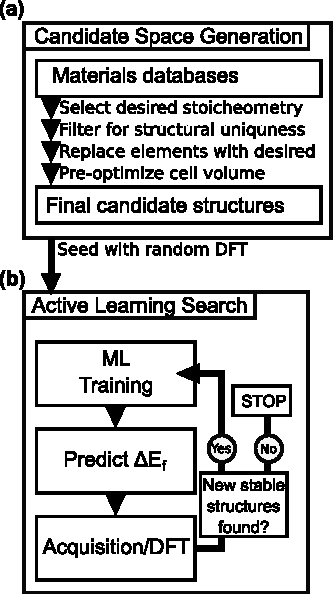
\includegraphics
  {02_figures/al_diagram/Surrogate_model_mine.pdf}
  }
\caption{\label{fig:all_diagram}
%
% Probably better to keep this caption really concise and refer to the text
Process flow diagram for the active learning accelerated algorithm. The procedure is composed of
(a) generation of the candidate set of considered crystal structures constructed from DFT materials databases and
(b) iterative active learning surrogate search of the candidate space.
}
\end{figure*}
% __|
% =========================================================
